\section{Hierarchy of Moment Equations for Shear Flow}
\begin{frame}{Ansatz for Derivation of Moment Equations}
	\scriptsize
    Consider approximation of the form
	\begin{align}
		\textcolor{cyan}{f(\textbf{x}, t, \phi, \theta) \approx f^N(\textbf{x},t,\phi,\theta) :=  \sum_{n=0}^{N} \sum_{i=-2n}^{2n} c^i_{2n}(\textbf{x},t) \cdot P^i_{2n}(\phi, \theta)}, \label{spectralmethod}
	\end{align}
	where $P^i_{2n}(\phi, \theta)$, $n = 0, \ldots, N$, $i = -2n, \ldots, 2n$
	\begin{itemize}
		\item are harmonic polynomial basis functions, i.e., the eigenfunctions of the Laplace-Beltrami operator with the eigenvalue $-2n(2n+1)$
		\pause
		\item form an orthonormal basis, wrt. the $L_2$-inner product on the sphere
		\begin{align*}
			(g,h)_{S^2} := \int_{0}^{2\pi} \int_{0}^{\pi} g(\phi, \theta) h(\phi, \theta) \cdot \sin(\theta) d\theta d\phi,
		\end{align*}
	\pause
	\item every square integrable function on $S^2$ can be expressed as a linear combination of spherical harmonics $f(\phi, \theta) = \sum^{\infty}_{n=0} \sum_{i=-n}^{n} c^i_{n} \cdot P^i_{n}(\phi, \theta)$.
	\end{itemize}
\end{frame}

\begin{frame}{Derivation of Moment Equations}
	\scriptsize
	We derive the moment equations by
	\begin{itemize}
		\item Insert ansatz $f^N =  \sum_{n=0}^{N} \sum_{i=-2n}^{2n} c^i_{2n}(x,t) \cdot P^i_{2n}(\phi, \theta)$ into kinetic equation
\begin{align*}
\sin\theta \partial_{t}f^N(x,t,\phi,\theta) + &  \textcolor{red}{\partial_x (\cos\phi \cos\theta \sin^2\theta f^N)} \\
	& 
	 =- \textcolor{blue}{\partial_\theta \left(w_x \sin^3 \theta \cos \phi f^N\right)} +\textcolor{blue}{D_{r} \left( \partial_\phi \left(\frac{1}{\sin \theta} \partial_\phi f^N \right) + \partial_\theta (\sin \theta \partial_\theta f^N) \right)}
\end{align*}
		\item Multiply consecutively with all basis functions used in the ansatz and integrate the resulting equations over the sphere
	\end{itemize}
\pause
The system of moment equations has the general form
\begin{align}
	\partial_t Q + \textcolor{red}{A\partial_x Q} = \textcolor{blue}{D(w_x)Q}+ \textcolor{blue}{D_rE Q},
\end{align}
where $Q=(c^0_0(x,t), c^{-2}_2(x,t), \ldots, c^{2N}_{2N}(x,t))^T$ represents the vector of the moments and \\
\vspace{2mm}
$A,D,E \in \mathbb{R}^{(N+1)(2N+1)x(N+1)(2N+1)}$.
\end{frame}

\begin{frame}{Derivation: A Closer Look}
\scriptsize
Consider 
\begin{align*}
	\textcolor{cyan}{\underbrace{\sin\theta \partial_{t}f^N(x,t,\phi,\theta)}_{[1]}} + &  \underbrace{\partial_x (\cos\phi \cos\theta \sin^2\theta f^N)}_{[2]} \\
	& 
	= -\partial_\theta \left(w_x \sin^3 \theta \cos \phi f^N\right) + D_{r} \left(\partial_\phi \left(\frac{1}{\sin \theta} \partial_\phi f^N \right) + \partial_\theta (\sin \theta \partial_\theta f^N) \right)
\end{align*}
\pause
For $k=0, \ldots, N$, $l=-2k, \ldots, 2k$ we obtain for term $[1]$
\begin{align*}
	&\int_{0}^{2\pi} \int_{0}^{\pi} \textcolor{cyan}{\sin\theta \partial_t \left(\sum_{n=0}^{N} \sum_{i=-2n}^{2n} c^i_{2n}(x,t) \cdot P^i_{2n}(\phi, \theta)\right)}P^l_{2k}(\phi, \theta) \\
	&= \sum_{n=0}^{N} \sum_{i=-2n}^{2n} \partial_t c^i_{2n}(x,t) \int_{0}^{2\pi} \int_{0}^{\pi} \sin\theta P^i_{2n}(\phi, \theta) P^l_{2k}(\phi, \theta) d\phi d\theta \\
	&=  \sum_{n=0}^{N} \sum_{i=-2n}^{2n} \partial_t c^i_{2n}(x,t) (P^i_{2n}(\phi, \theta) P^l_{2k}(\phi, \theta))_{S^2} =  \sum_{n=0}^{N} \sum_{i=-2n}^{2n} \partial_t c^i_{2n}(x,t) \cdot \delta_{n,k} \delta_{i,l} \\
	&= \partial_t c^l_{2k}(x,t)
\end{align*}
\pause
This corresponds to this term
$\textcolor{cyan}{\partial_t Q} + A\partial_x Q = D(w_x)Q+ D_rE Q$.
\end{frame}

\begin{frame}
	\scriptsize
Consider term [2]
\begin{align*}
	\underbrace{\sin\theta \partial_{t}f^N(x,t,\phi,\theta)}_{[1]} + &  \textcolor{cyan}{\underbrace{\partial_x (\cos\phi \cos\theta \sin^2\theta f^N)}_{[2]}} \\
	& 
	= -\partial_\theta \left(w_x \sin^3 \theta \cos \phi f^N\right) + D_{r} \left(\partial_\phi \left(\frac{1}{\sin \theta} \partial_\phi f^N \right) + \partial_\theta (\sin \theta \partial_\theta f^N) \right)
\end{align*}
\pause
This represents the term
$\partial_t Q + \textcolor{cyan}{A\partial_x Q} =  D(w_x)Q+ D_rEQ$ \\
\vspace{2mm}
For $N=1$ the matrix $A$ has the form
\begin{figure}[H]
		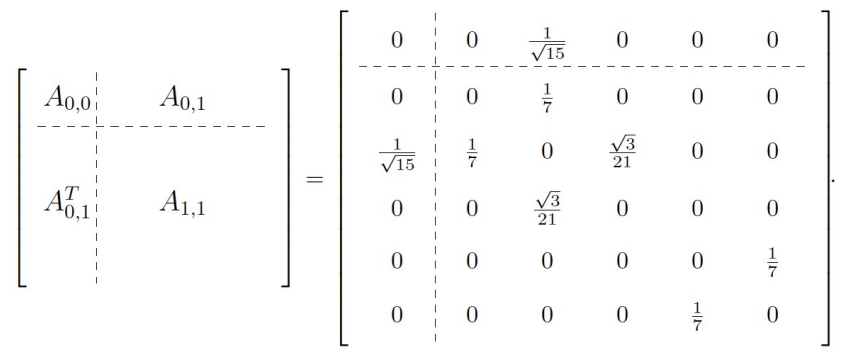
\includegraphics[scale=0.5]{Bilder/MatrixA}
\end{figure}
\end{frame}


\begin{comment}
	For $N=1$ the matrix $A$ has the form
	\begin{equation}
		\left[\begin{array}{c:c}
			A_{0,0} & A_{0,1} \\
			\hdashline A_{0,1}^T & A_{1,1}
		\end{array}\right]=\left[\begin{array}{c:ccccc}
			0 & 0 & \frac{1}{\sqrt{15}} & 0 & 0 & 0 \\
			\hdashline 0 & 0 & \frac{1}{7} & 0 & 0 & 0 \\
			\frac{1}{\sqrt{15}} & \frac{1}{7} & 0 & \frac{\sqrt{3}}{21} & 0 & 0 \\
			0 & 0 & \frac{\sqrt{3}}{21} & 0 & 0 & 0 \\
			0 & 0 & 0 & 0 & 0 & \frac{1}{7} \\
			0 & 0 & 0 & 0 & \frac{1}{7} & 0
		\end{array}\right] .
	\end{equation}
\end{comment}

%%%%%%%%%%%%%%%%%%%%%%%%%%%%%%%%%%%%%%%%%%%%%%%%%%%%%%%%%%%%%%%%%
%%%%%%%%%%%%%%%%% Struktur Matrix A N=2 machen %%%%%%%%%%%%%%%%%%
%%%%%%%%%%%%%%%%%%%%%%%%%%%%%%%%%%%%%%%%%%%%%%%%%%%%%%%%%%%%%%%%%


\begin{frame}
	\scriptsize
	For N = 2 the symmetric matrix A has the structure
\begin{figure}[H]
	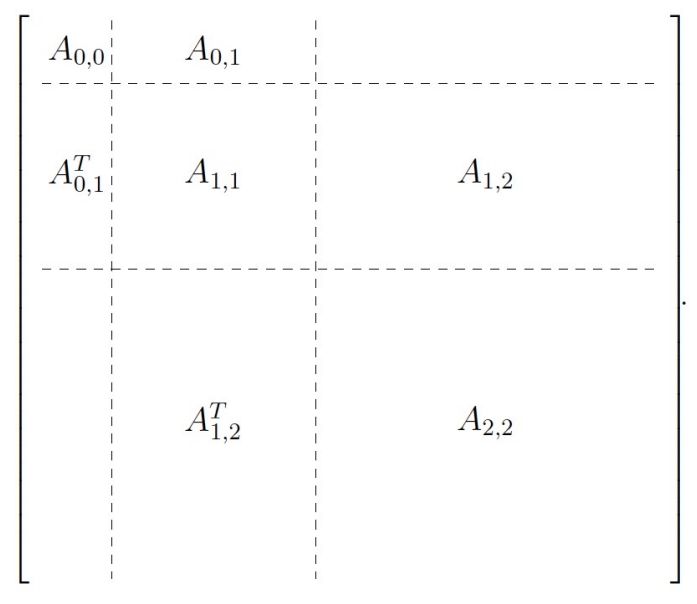
\includegraphics[scale=0.5]{Bilder/MatrixAN=2}
\end{figure}
\textcolor{cyan}{For any N the system of moment equations is hyperbolic.}
\end{frame}

\begin{frame}
		\scriptsize
Now consider the remaining terms:
	\begin{align*}
		\sin\theta \partial_{t}f^N(x,t,\phi,\theta) &+ \partial_x (\cos\phi \cos\theta \sin^2\theta f^N) \\
		&= \textcolor{cyan}{\underbrace{-\partial_\theta \left(w_x \sin^3 \theta \cos \phi f^N\right)}_{[3]} + \underbrace{D_{r} \left(\partial_\phi \left(\frac{1}{\sin \theta} \partial_\phi f^N \right) + \partial_\theta (\sin \theta \partial_\theta f^N) \right)}_{[4]}}.
	\end{align*}
\pause
\begin{itemize}
	\item Term $[4]$ corresponds to the Laplace-Beltrami operator,  resulting in $\textcolor{cyan}{D_r E Q}$, where the matrix $E$ is a diagonal matrix with the Laplace-Beltrami eigenvalues. 
	\pause
	\item Term $[3]$: We apply the same approach by inserting the ansatz for $f$ and projecting onto the polynomials, resulting in $\textcolor{cyan}{D(w_x)Q}$.
\end{itemize}
\vspace{5mm}
The system of moment equations:
$\partial_t Q + A\partial_x Q =  D(w_x)Q+ D_rEQ$. 
\end{frame}

\begin{comment}
\begin{frame}{Hierarchy of Moment Equations for Shear Flow}
\scriptsize
For $N=1$ we obtain 
\begin{equation}
	\begin{aligned}
		&\partial_t Q + \textcolor{red}{
			\begin{pmatrix}
				0 & 0 & \frac{\sqrt{15}}{15} & 0 & 0 & 0 \\
				0 & 0 & \frac{1}{7} & 0 & 0 & 0 \\
				\frac{\sqrt{15}}{15} & \frac{1}{7} & 0 & \frac{\sqrt{3}}{21} & 0 & 0 \\
				0 & 0 & \frac{\sqrt{3}}{21} & 0 & 0 & 0 \\
				0 & 0 & 0 & 0 & 0 & \frac{1}{7} \\
				0 & 0 & 0 & 0 & \frac{1}{7} & 0
		\end{pmatrix} \cdot \partial_x Q} \\
		&= \textcolor{blue}{
			\begin{pmatrix}
				0 & 0 & 0 & 0 & 0 & 0 \\
				0 & -6D_r & \frac{2}{7}w_x & 0 & 0 & 0 \\
				-\frac{\sqrt{15}}{5}w_x & -\frac{5}{7}w_x & -6D_r & \frac{3\sqrt{3}}{7}w_x & 0 & 0 \\
				0 & 0 & -\frac{4\sqrt{3}}{7}w_x & -6D_r & 0 & 0 \\
				0 & 0 & 0 & 0 & -6D_r & -\frac{5}{7} w_x \\
				0 & 0 & 0 & 0 & \frac{2}{7}w_x & -6D_r
			\end{pmatrix} Q }.
	\end{aligned}
\end{equation}
\end{frame}
\end{comment}



